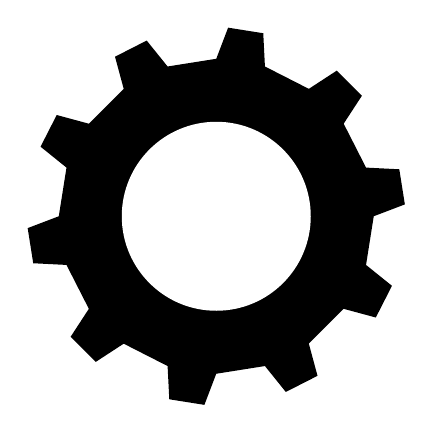
\begin{tikzpicture}[scale=2]
    % Gear parameters
    \def\teeth{10}
    \def\Iradius{0.6}
    \def\radius{1}
    \def\Oradius{1.2}
    \def\toothheight{0.2}
    \def\toothangle{360/\teeth}
    \def\offset{0.1*\toothangle}

    % Start drawing the gear
    \path[fill=\gearColor]
    % Start at angle 0
    (0:{\radius})
    \foreach \i in {1,...,\teeth} {  
        -- ({\toothangle*(\i - 1) + \offset}:\Oradius) % Goes out
        -- ({\toothangle*(\i - 1) + \toothangle/2 - \offset}:\Oradius) % Spin outer
        -- ({\toothangle*(\i - 1) + \toothangle/2}:\radius) % Go in
        -- ({\toothangle*(\i)}:\radius) % Spin inner
        % -- ({\toothangle*(\i - 1) + \toothangle/2}:{\radius + \toothheight}) % tip of tooth
        % -- ({\toothangle*(\i - 1) + \toothangle}:{\radius})               % back to base circle
    } -- cycle;

    % Optional: center hole
    \fill[white] (0,0) circle (\Iradius);

\end{tikzpicture}